\chapter{A new test case for exciting the Lorenz computational mode}
\label{ch:cp}

\begin{highlights}
{\Large Highlights}
\begin{itemize}
	\item A new idealised two-dimensional test case reveals spurious grid-scale waves excited by the Lorenz computational mode
	\item The Charney--Phillips staggering is generalised for arbitrary meshes that reduces to classical Charney--Phillips on traditional meshes
	\item A new fully compressible Euler model that implements the generalised Charney--Phillips formulation is free from spurious grid-scale waves
\end{itemize}
\end{highlights}

The Lorenz computational mode arises from having one too many degrees of freedom in the Lorenz staggering of variables, and it is often excited by thermal forcing, producing spurious, vertical, grid-scale waves \citep{schneider1987,arakawa-konor1996}.
In the Lorenz staggering, the pressure and vertical velocity variables are staggered, with the thermodynamic variable collocated with the pressure variable \citep{lorenz1960}.
Vertical averaging of the thermodynamic variable in calculating vertical momentum means that these grid-scale waves persist because they become invisible to the model \citep{arakawa-konor1996}.
Spurious grid-scale waves have been attributed to the Lorenz computational mode in the Global Environmental Multiscale 3 model \citep{girard2014}, and the Korea Institute of Atmospheric Prediction Systems Integrated Model \citep{yi-park2017} amongst others, and these non-physical waves can lead to spurious rainfall in atmospheric models \citep{hollingsworth1995}, inaccurate simulations of idealised hurricanes \citep{zhu-smith2003}, and spurious instabilities in ocean models \citep{bell-white2017}.

The computational mode can be at least partially controlled by using sufficient vertical diffusion \citep{chang1992,zadra2004}, or by using a higher-order vertical discretisation \citep{untch-hortal2004,guerra-ullrich2016,yi-park2017}, but the computational mode can only be properly eliminated by choosing an alternative staggering of variables that removes the extra degree of freedom.
One such alternative is the Charney--Phillips staggering \citep{charney-phillips1953}, in which the thermodynamic variable is collocated with vertical velocity, avoiding any vertical averaging in calculating vertical momentum.
Models that use a Charney--Phillips staggering include the Met Office Unified Model \citep{davies2005}, the Global Environmental Multiscale 4 model \citep{girard2014}, and the Global/Regional Assimilation and Prediction System \citep{yang2007}.
\citet{thuburn-woolings2005} exhaustively tested different combinations of vertical coordinates, prognostic variables and their staggerings, and found that a Charney--Phillips staggering has better dispersion properties than a Lorenz staggering for any given choice of vertical coordinate and prognostic variables.
Numerical experiments performed by \citet{cullen1997} revealed that a model with a Charney--Phillips staggering reduced spurious gravity waves and had better geostrophic adjustment compared to \TODO{the same?} model with a Lorenz staggering.

While the Charney--Phillips staggering avoids vertical averaging of the thermodynamic variable in calculating vertical momentum, \citet{davies2005} notes that horizontal pressure gradient calculations can involve vertical averaging which is inaccurate in the lowest layers where there are strong temperature gradients.
\citet{holdaway2013a} note that, in calculating the Richardson number for boundary layer schemes, averaging that is necessary with the Charney--Phillips staggering that is avoided by using a Lorenz staggering.

Previous studies have used a variety of test cases to compare different model variants using Lorenz and Charney--Phillips staggering.
One of the earliest comparisons was made by \citet{arakawa-moorthi1988} who found that, without additional diffusion, their numerical solutions of a baroclinic instability test were dominated by short-wave noise.
Later, \citet{arakawa-konor1996} performed the same test to find that a model using a Charney--Phillips staggering did not suffer from spurious noise, with the model needing no additional diffusion.
In the same study, \citet{arakawa-konor1996} proposed new test cases that use thermal forcing to excite the Lorenz computational mode.
The new test cases were performed using an idealised, vertically discrete model and clearly reveal spurious grid-scale waves that grow and persist throughout the simulation.
Based on the work of \citet{arakawa-konor1996}, \citet{untch-hortal2004} developed a new test case, using thermal forcing to excite spurious grid-scale waves in a 600-day integration of a global, 3D model.

We propose a new, idealised two-dimensional test case, also based on the work of \citet{arakawa-konor1996}, to compare the accuracy of models using Lorenz or Charney--Phillips staggerings.  The new test case intended to aid in the development and intercomparison of modern, nonhydrostatic dynamical cores, and uses a coarse two-dimensional mesh specified in Cartesian coordinates.
We compare test results between the fully compressible Euler model with a Lorenz staggering (section~\ref{sec:slanted:exnerFoamH}), and a variant of this same more that includes a new generalisation of the Charney--Phillips staggering for arbitrary meshes.

After describing the generalised Charney--Phillips formulation in section~\ref{sec:cp:method}, we compare Lorenz and generalised Charney--Phillips model variants in section~\ref{sec:cp:schaerWaves} using the standard mountain waves test case specified by \citet{schaer2002}.
Section~\ref{sec:cp:arakawaKonor} presents the new test case based on \citet{arakawa-konor1996}. We verify that the Lorenz computational mode is excited using the fully compressible Euler model with a Lorenz staggering.  Using the generalised Charney--Phillips model variant, the sensitivity to mesh distortions is explored.  Finally, in section~\ref{sec:cp:advection}, we extract the transport scheme from the generalised Charney--Phillips model variant and examine numerical errors using transport tests on distorted and undistorted meshes.

\section{Generalising the Charney–Phillips staggering for arbitrary meshes}
\label{sec:cp:method}

The generalisation of the Lorenz staggering for arbitrary meshes is straightforward \citep{weller-shahrokhi2014} but this is not true for the Charney--Phillips staggering, which is only suitable for structured meshes with cells stacked in columns.
On a finite volume mesh, variables are ordinarily placed at cell centres or cell faces.
In the Charney--Phillips staggering, the thermodynamic variable is placed at only those cell faces that lie on the vertical coordinate surfaces, and vertically-oriented faces have no thermodynamic information.
This existing staggering is unsuitable for arbitrary finite volume meshes because faces can have any orientation.

A generalised Charney--Phillips staggering will be particularly relevant to atmospheric models that use vertical mesh refinement techniques.
Mesh refinement has received growing attention in atmospheric modelling literature because it could enable atmospheric models to produce more accurate forecasts with less computation \citep{behrens2006,jablonowski2009}.
While much of the literature concentrates on horizontal mesh refinement, some investigations have been made into vertical refinement on two-dimensional $x$--$z$ Cartesian planes:
\citet{mueller2013} have used conforming refinement of triangular meshes for simulating the standard rising bubble and density current test cases, \citet{vanhooft2018} have used block-structured adaptive mesh refinement for direct numerical simulations of the atmospheric boundary layer, and \citet{yamazaki-satomura2012} have used nonconforming block-refinement to better resolve the atmosphere immediately above idealised mountains.

According to \citet{thuburn-woolings2005}, the vertical discretisation used by \citet{yamazaki-satomura2012} supports computational modes and instabilities, although these errors were not excited by the test cases performed by \citet{yamazaki-satomura2012}.
The Charney--Phillips staggering is not susceptible to such errors, but we are not aware of any existing literature that combines mesh refinement with a Charney--Phillips staggering.
By allowing for any mesh structure, a generalised Charney--Phillips formulation should be suitable for any type of mesh, including conforming and non-conforming mesh refinement, terrain-following meshes, cut cell meshes and slanted cell meshes.

\subsection{Generalised Charney--Phillips formulation}

\begin{figure}
	\centering
	\documentclass[tikz]{standalone}
\usepackage{times}
\usepackage{bm}
\begin{document}
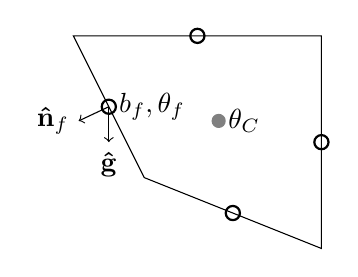
\begin{tikzpicture}[
  scale=0.45,
  cpnt/.style={fill=gray}
]

\draw (2,3) -- (0,7) -- (7,7) -- (7,1) -- (2,3);

\path [cpnt] (4.1,4.6) circle [radius=0.2] node [right] {$\theta_C$};

\draw [thick] (7,4) circle [radius=0.2];
\draw [thick] (4.5,2) circle [radius=0.2];
\draw [thick] (3.5,7) circle [radius=0.2];
\draw [thick] (1,5) circle [radius=0.2] node [right] {$b_f, \theta_f$};

\draw [->] (1,5) -- (0.15,4.6) node [left] {$\mathbf{\hat{n}}_f$};
\draw [->] (1,5) -- (1,4) node [below] {$\mathbf{\hat{g}}$};

\end{tikzpicture}
\end{document}

	\caption{A quadrilateral cell with the prognostic thermodynamic variable $b_f$ stored at face centres marked by open circles.
	$b_f$ is calculated from the potential temperature $\theta_f$ such that $b_f = \theta_f \unitg \cdot \unitn_f$ where $\unitn_f$ is the unit vector outward normal to face $f$, and $\unitg$ is the unit vector of gravitational acceleration.
	The potential temperature at the cell centre, $\theta_C$, is reconstructed from surrounding values of $b_f$ using equation~\eqref{eqn:cp:reconstruct}.}
	\label{fig:cp:staggering}
\end{figure}

The generalised Charney--Phillips model is a new variant of the fully compressible Euler model with a Lorenz staggering, as documented by \citet{weller-shahrokhi2014} and summarised in section~\ref{sec:slanted:exnerFoamH}.
The model variant uses a newly-formulated generalisation of the Charney--Phillips staggering for arbitrary meshes.
The primary difference between the Lorenz and Charney--Phillips formulations is their treatment of the prognostic thermodynamic variable: the generalised Charney--Phillips formulation stores the prognostic thermodynamic variable $b_f$ at all cell faces such that $b_f = \theta_f \unitg \cdot \unitn_f$ where $f$ is a face, $\theta_f$ is the potential temperature at the face, $\unitg$ is the unit vector of gravitational acceleration and $\unitn_f$ is the unit vector that is outward normal to the face.
This arrangement is illustrated in figure~\ref{fig:cp:staggering}.
To transport the thermal field, first, potential temperature is transported in advective form using first-order time-stepping,
\begin{align}
	\theta_f^{n+1} &= \theta_f^n - \Delta t \uf \cdot \left( \nabla_c \theta_f^{\ell} \right)_F \label{eqn:cp:advection}
\end{align}
where $\theta_f^{n+1}$ is the value of $\theta_f$ at the new time-step, $\theta_f^\ell$ is the lagged value from the previous time-stepping iteration, $\uf$ is the wind, $\left( \cdot \right)_F$ denotes an interpolation from cell centres to faces, and $\nabla_c$ denotes a cell centre gradient \citep{weller-shahrokhi2014}.
Next, $b_f$ is calculated such that $b_f = \theta_f \unitg \cdot \unitn_f$.  
On a Cartesian mesh with no diagonal faces, $b_f$ is zero for entirely vertical faces and $b_f = \theta_f$ for entirely horizontal faces.

Potential temperature at the cell centre is reconstructed from bordering faces,
\begin{align}
	\theta_C &= \unitg \cdot \left( \sum_{f \in c} \unitn_f \Sf \right)^{-1} \cdot \sum_{f \in c} \Sf b_f \label{eqn:cp:reconstruct}
\end{align}
where $\theta_C$ is the reconstructed potential temperature.  On a Cartesian mesh with no diagonal faces, $\theta_C$ is simply a linear interpolation from the face values immediately above and below the cell centre.

Finally, $\theta_f$ is recalculated from $b_f$ and $\theta_C$,
\begin{align}
	\theta_f &:= \Mag{ \unitg \cdot \unitn_f \theta_f} + \left( 1 - \Mag{\unitg \cdot \unitn_f } \right) \left( \theta_C \right)_F \text{.}
\end{align}
This ensures that values of $\theta_f$ on vertical faces is calculated from nearby $b_f$ values and is not retained across time-steps.

The generalised Charney--Phillips model variant makes two other modifications to the Lorenz model variant in order to simplify implementation: first, gravity waves are treated explicitly and, second, first-order Euler semi-implicit time-stepping is used with deferred correction of explicit terms (equation~\ref{eqn:cp:advection}).


\section{Sch\"{a}r mountain waves test}
\label{sec:cp:schaerWaves}

Chapter~\ref{ch:slanted} assessed a finite volume model of the fully compressible Euler equations with a Lorenz staggering using a test case with a stratified atmosphere initially at rest above an isolated mountain.
We now turn our attention to a transport-dominated test case that presents a challenge to the transport schemes within the dynamical model.
As specified by \citet{schaer2002}, the test prescribes flow over idealised terrain with small-scale and large-scale undulations that induce propagating and evanescent gravity waves.
We use the test to compare results from the two finite volume model variants with Lorenz and generalised Charney--Phillips staggerings against the reference solution from \citet{melvin2010}.

Following \citet{melvin2010}, the domain is \SI{300}{\kilo\meter} wide and \SI{30}{\kilo\meter} high, and the mesh spacing is $\Delta x = \SI{500}{\meter}$ and $\Delta z^\star = \SI{300}{\meter}$.
The mountain profile has the same form as equation~\eqref{eqn:resting:mountain}, but the mountain waves test has a lower peak mountain height of $h_0 = \SI{250}{\meter}$.  As in the resting atmosphere test (section~\ref{sec:slanted:resting}), $a = \SI{5}{\kilo\meter}$ is the mountain half-width and $\lambda = \SI{4}{\kilo\meter}$ is the wavelength.

A uniform horizontal wind $(u, w) = (10, 0)\:\si{\meter\per\second}$ is prescribed in the domain interior and at the inlet boundary.  No normal flow is imposed at the top and bottom boundaries and the velocity field has a zero gradient outlet boundary condition.

The initial thermodynamic conditions have constant static stability with $N = \SI{0.01}{\per\second}$ everywhere such that
\begin{align}
	\theta(z) = \theta_0 \exp \left( \frac{N^2}{g} z \right) \label{eqn:cp:schaerWaves:thermal-profile}
\end{align}
where the temperature at $z=0$ is $\theta_0 = \SI{288}{\kelvin}$.
Potential temperature values are prescribed at the inlet and upper boundary using equation~\eqref{eqn:cp:schaerWaves:thermal-profile}, and a zero gradient boundary condition is applied at the outlet.
At the ground, fixed gradients are imposed by calculating the component of $\nabla \theta$ normal to each face using the vertical derivative of equation~\eqref{eqn:cp:schaerWaves:thermal-profile}.
For the Exner function of pressure, hydrostatic balance is prescribed on top and bottom boundaries and the inlet and outlet are zero normal gradient.

Sponge layers are added to the upper \SI{10}{\kilo\meter} and leftmost \SI{10}{\kilo\meter} at the inlet boundary to damp the reflection of waves.
The damping term \(\mu\) in the momentum equation \eqref{eqn:exnerFoam:momentum} is a function adapted from \citet{melvin2010} such that
\begin{subequations}
\begin{align}
	\mu(x, z) &= \mu_\mathrm{upper} + \mu_\mathrm{inlet} \\
	\mu_\mathrm{upper}(z) &= \begin{cases}
		\overline{\mu} \sin^2 \left( \frac{\pi}{2} \frac{z - z_B}{H - z_B} \right) & \enskip \text{if $z \geq z_B$,} \\
		0 & \enskip \text{otherwise,} \\
	\end{cases} \\
	\mu_\mathrm{inlet}(x) &= \begin{cases}
		\overline{\mu} \sin^2 \left( \frac{\pi}{2} \frac{x_I - x}{x_I - x_0} \right) & \enskip \text{if $x < x_I$,} \\
		0 & \enskip \text{otherwise,}
	\end{cases}
\end{align}%
\end{subequations}
where $\overline{\mu} = \SI{1.2}{\per\second}$ is the damping coefficient, $z_B = \SI{20}{\kilo\meter}$ is the bottom of the sponge layer, $H = \SI{30}{\kilo\meter}$ is the top of the domain, $x_0 = \SI{-150}{\kilo\meter}$ is the leftmost limit of the domain and $x_I = \SI{-140}{\kilo\meter}$ is the rightmost extent of the inlet sponge layer.
The sponge layer is active only on entirely horizontal faces so that only vertical momentum is damped.
Note that, while the domain itself is \SI{30}{\kilo\meter} in height, for the purposes of generating basic terrain-following meshes, the domain height is set to \SI{20}{\kilo\meter} because the sponge layer occupies the uppermost \SI{10}{\kilo\meter}.

\begin{figure}
	\centering
	\begin{subfigure}{0.55\textwidth}
		\centering
		\caption{Lorenz staggering, linearUpwind transport}
		\label{fig:cp:schaerWaves:w:linearUpwind}
		\includegraphics{thesis/cp/schaerWaves/fig-btf-300dz-linearUpwind-w.pdf}
	\end{subfigure}
	\begin{subfigure}{0.44\textwidth}
		\centering
		\caption{Lorenz staggering, cubicFit transport}
		\label{fig:cp:schaerWaves:w:cubicFit}
		\includegraphics{thesis/cp/schaerWaves/fig-btf-300dz-cubicFit-w.pdf}
	\end{subfigure}
	\\
	\vspace*{1em}
	%
	\begin{subfigure}{0.55\textwidth}
		\centering
		\caption{Generalised Charney--Phillips staggering}
		\label{fig:cp:schaerWaves:w:cp}
		\includegraphics{thesis/cp/schaerWaves/fig-btf-300dz-cp-w.pdf}
	\end{subfigure}
	\begin{subfigure}{0.44\textwidth}
		\centering
		\caption{Reference solution by \citet{melvin2010}}
		\label{fig:cp:schaerWaves:w:melvin}
		\raisebox{0.2in}{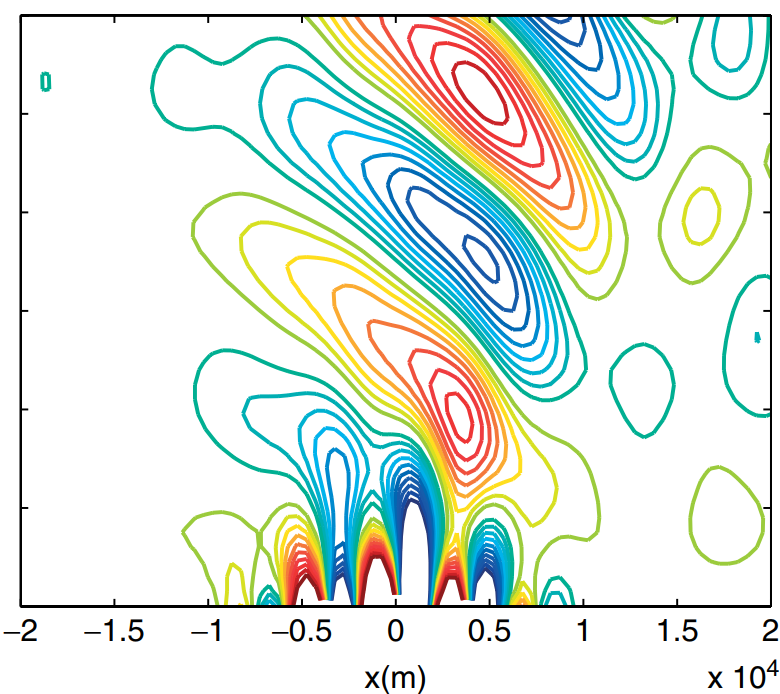
\includegraphics[height=1.9in]{cp/schaerWaves/melvin2010-w-mass-conserving-sisl.png}}
	\end{subfigure}
	\caption{Vertical velocities at the end of integration of the Sch\"{a}r mountain waves test case.
	Results obtained using a basic terrain-following mesh and Lorenz staggering, with potential temperature and momentum transported by (\subcaptionref{fig:cp:schaerWaves:w:linearUpwind}) the linearUpwind scheme and
	(\subcaptionref{fig:cp:schaerWaves:w:cubicFit}) the cubicFit scheme, and (\subcaptionref{fig:cp:schaerWaves:w:cp}) using a basic terrain-following mesh and generalised Charney--Phillips staggering.
	For comparison, (\subcaptionref{fig:cp:schaerWaves:w:melvin}) provides a reference solution obtained with a mass-conserving semi-implicit semi-Lagrangian model \citep{melvin2010}.
	Contours are plotted every \SI{0.05}{\meter\per\second}.  In figures (\subcaptionref{fig:cp:schaerWaves:w:linearUpwind}), (\subcaptionref{fig:cp:schaerWaves:w:cubicFit}) and (\subcaptionref{fig:cp:schaerWaves:w:cp}), ascending velocities are marked by solid black lines and descending velocities are marked by dashed red lines.
Only the lowest \SI{12}{\kilo\meter} in the central region of the domain is shown.  The entire domain is \SI{300}{\kilo\meter} wide and \SI{30}{\kilo\meter} high.
	}
	\label{fig:cp:schaerWaves:w}
\end{figure}

The test is integrated forward by five hours using a time-step of \SI{8}{\second}.  At the end of the simulation, gravity waves are apparent in the contours of vertical velocity (figure~\ref{fig:cp:schaerWaves:w}).
Results are presented for the Lorenz model variant, with momentum and potential temperature being transported using the linearUpwind scheme (figure~\ref{fig:cp:schaerWaves:w:linearUpwind}) and the cubicFit scheme (figure~\ref{fig:cp:schaerWaves:w:cubicFit}), and for the generalised Charney--Phillips model variant (figure~\ref{fig:cp:schaerWaves:w:cp}), and all are in general agreement with the reference solution from \citet{melvin2010}, reproduced in figure~\ref{fig:cp:schaerWaves:w:melvin}.
All four results presented in figure~\ref{fig:cp:schaerWaves:w} were obtained using the same basic terrain-following mesh.

Spurious distortions are visible in the vertical velocity contours using the Lorenz model variant and the linearUpwind transport scheme (figure~\ref{fig:cp:schaerWaves:w:linearUpwind}), and similar error structures have been found in previous studies that were attributed to numerical errors associated with basic terrain-following mesh distortions \citep{schaer2002,klemp2003}.
In agreement with these previous findings, we find that spurious gravity wave distortions can be avoided by switching from a basic terrain-following mesh to a slanted cell mesh or cut cell mesh (results not shown).
We also find that spurious gravity wave distortions can be avoided by transporting momentum and potential temperature on a basic terrain-following mesh using the cubicFit scheme (figure~\ref{fig:cp:schaerWaves:w:cubicFit}).
Avoiding such spurious gravity waves distortions using either approach produces solutions that closely match the reference solution (figure~\ref{fig:cp:schaerWaves:w:melvin}).
Given these results, we can attribute spurious gravity wave distortions to transport scheme errors associated with flow that is misaligned with mesh layers.
Unlike the results obtained by \citet{shaw-weller2016} that used an older formulation of the cubicFit scheme, potential temperature errors are negligible for all types of mesh when using the most recent formulation of the cubicFit scheme documented in chapter~\ref{ch:cubicFit}.

As seen in figure~\ref{fig:cp:schaerWaves:w:cp}, the generalised Charney--Phillips model variant produces gravity waves with spurious distorted structures similar to those obtained using the Lorenz model variant with the linearUpwind scheme (figure~\ref{fig:cp:schaerWaves:w:linearUpwind}).
In addition, as evidenced by the density of vertical velocity contour lines in figure~\ref{fig:cp:schaerWaves:w:cp}, the generalised Charney--Phillips model variant produces gravity wave amplitudes that are too large compared to the reference solution.

In summary, all solutions obtained here are in general agreement with the reference solution from \citet{melvin2010}.
However, on the basic terrain-following mesh, numerical errors lead to spurious gravity wave distortions using the generalised Charney--Phillips model variant and using the Lorenz model variant with momentum and potential temperature transported by the linearUpwind scheme.
Using the more accurate cubicFit scheme in the Lorenz model variant produces the correct solution on the basic terrain-following mesh that is free from any spurious gravity wave distortions.

Knowing that an improved transport scheme was responsible for the improved gravity wave solution using the Lorenz model variant, we conjecture that the generalised Charney--Phillips model variant produces less accurate results because the model uses a transport scheme that is insufficiently accurate.
In the next section we perform a further comparison between Lorenz and generalised Charney--Phillips model variants using a new test case to excite the Lorenz computational mode.


\section{A two-dimensional standing waves test case}
\label{sec:cp:arakawaKonor}

\TODO{
\begin{itemize}
	\item Plot: horizontal edgeGrading, vertical edgeGrading
	\item Plot: conservation of internal energy and total energy time series, ExnerFoamH and ExnerFoamCP, uniform mesh, horizontal edgeGrading, vertical edgeGrading
	\item Conclusion: the test excites the Lorenz computational mode with ExnerFoamH
	\item Conclusion: ExnerFoamCP eliminates computational mode
	\item Conclusion: edgeGrading reveals lack of conservation, due to advective form transport scheme?
\end{itemize}
}

\TODO{a little intro.  say again that all this is based on the standing waves test case by \citet{arakawa-konor1996}.}

The domain is \SI{30}{\kilo\meter} high and \SI{600}{\kilo\meter} wide between the outermost faces, and the mesh spacing is $\Delta x = \SI{10}{\kilo\meter}$ and $\Delta z = \SI{1}{\kilo\meter}$.  The lower boundary is flat with no mountain profile.
The upper and lower boundaries are no normal flow, and the domain is horizontally periodic.

The initial potential temperature profile is the sum of a stably-stratified profile and a grid-scale perturbation near the ground.
The stably-stratified profile has $\theta(z = 0) = \SI{250}{\kelvin}$ and a constant static stability with Brunt-V\"ais\"al\"a frequency $N = \SI{0.02}{\per\second}$.
The potential temperature perturbation $\theta'$ is defined as
\begin{subequations}
\label{eqn:cp:arakawaKonor:theta-perturbation}
\begin{align}
	\theta' &= \begin{cases} S \theta'_0 \sin(\frac{2 \pi x}{\lambda}) & \text{if } \Mag{x} \leq \frac{\lambda}{2} \\
		0 & \text{otherwise} \\
	\end{cases} \\
\shortintertext{where}
	S &= \begin{cases}
		-1 & \text{if } \SI{1}{\kilo\meter} <= z < \SI{2}{\kilo\meter} \\
		1 & \text{if } \SI{2}{\kilo\meter} <= z < \SI{3}{\kilo\meter} \\
		0 & \text{otherwise} \\
	\end{cases}
\end{align}
\end{subequations}
and the maximum amplitude $\theta'_0 = \SI{0.5}{\kelvin}$ and the wavelength $\lambda = \SI{100}{\kilo\meter}$.
Using a Lorenz staggering, this arrangement produces grid-scale waves in the central region of the domain in two layers near the ground (figure~\ref{fig:cp:arakawaKonor:theta_diff:initial}).
Using a generalised Charney--Phillips staggering, the perturbation is non-zero on the lowest two interior mesh layers above the lower boundary (not shown).
The definition given by equation~\eqref{eqn:cp:arakawaKonor:theta-perturbation} ensures that the potential temperature perturbation integrated over the domain is zero.

At the upper and lower boundaries, zero gradients are imposed on the potential temperature field for the Lorenz model variant; for the Charney--Phillips model variant, fixed potential temperature values are prescribed using equation~\ref{eqn:cp:schaerWaves:thermal-profile}.
The Exner function of pressure is calculated so that it is in discrete hydrostatic balance.

A sponge layer is added to the upper \SI{10}{\kilo\meter}.  The damping function is given by
\begin{align}
	\mu(z) &= \begin{cases}
		\overline{\mu} \sin^2 \left( \frac{\pi}{2} \frac{z - z_B}{H - z_B} \right) & \text{if } z \geq z_B \\
		0 & \text{otherwise} \\
	\end{cases}
\end{align}
where $\overline{\mu} = \SI{1.2}{\per\second}$ is the damping coefficient, $z_B = \SI{20}{\kilo\meter}$ is the bottom of the sponge layer and $H = \SI{30}{\kilo\meter}$ is the top of the domain.
The sponge layer is only active on faces whose normal is vertical so that it damps vertical momentum only.

The test is integrated forward by 48 hours using a time-step of $\Delta t = \SI{25}{\second}$.

\begin{figure}
	\centering
	\begin{subfigure}{0.38\textwidth}
		\vspace*{1.1em}
		\includegraphics{arakawaKonor-uniform-lorenz/0/theta_diff.pdf}
		\caption{Initial perturbation with a Lorenz staggering}
		\label{fig:cp:arakawaKonor:theta_diff:initial}
	\end{subfigure}
	\begin{subfigure}{0.3\textwidth}
		\includegraphics{arakawaKonor-uniform-lorenz/172800/theta_diffS.pdf}
		\caption{Lorenz solution}
		\label{fig:cp:arakawaKonor:theta_diff:lorenz}
	\end{subfigure}
	\begin{subfigure}{0.3\textwidth}
		\vspace*{1.1em}
		\includegraphics{arakawaKonor-uniform-cp/172800/theta_diffS.pdf}
		\caption{Generalised Charney--Phillips solution}
		\label{fig:cp:arakawaKonor:theta_diff:cp}
	\end{subfigure}
%
\vspace{0.5em}
\includegraphics[height=5in,angle=270]{arakawaKonor-uniform-lorenz/arakawaKonor-initial-theta_diff-colorBar.eps}
%
	\caption{Differences in potential temperature for the standing waves test case.
	(\subcaptionref{fig:cp:arakawaKonor:theta_diff:initial}) a grid-scale potential temperature perturbation near the surface is added to an initial, stably-stratified profile.
The difference between the initial, unperturbed, stably-stratified potential temperature profile and the final solution are shown using
	(\subcaptionref{fig:cp:arakawaKonor:theta_diff:lorenz}) the Lorenz model variant, and 
	(\subcaptionref{fig:cp:arakawaKonor:theta_diff:cp}) the generalised Charney--Phillips model variant.
Only the lowest \SI{20}{\kilo\meter} in the central region of the domain is shown.  The entire domain is \SI{600}{\kilo\meter} wide and \SI{30}{\kilo\meter} high.
	}
	\label{fig:cp:arakawaKonor:theta_diff}
\end{figure}

\TODO{discuss uniform results}

\TODO{introduce edgeGrading meshes: should we specify these with a Jacobian rather than OpenFOAM's edgeGrading notation?}


\section{Horizontal transport on distorted Charney--Phillips meshes}
\label{sec:cp:advection}
\TODO{
\begin{itemize}
	\item Test: horizontal advection; advectiveFoamF, advectionFoam with linear interp, advectionFoam with linearUpwind interp; measure l2 and linf errors (s.t. they can be compared with cell-centred, C-grid results); uniform and edgeGraded meshes
	\item Plot: error fields, analytic+numerical contours of final solution, which schemes and which meshes? too many combinations to plot all of them
	\item Plot: time-series of conservation, ExnerFoamH and ExnerFoamCP, uniform mesh, horizontal edgeGrading, vertical edgeGrading
	\item Conclusion: advection is conservative on uniform meshes, non-conservative on non-uniform meshes
	\item Conclusion: advectiveFoamF errors are comparable to advectionFoam with linear interpolation?
	\item Conclusion: advectiveFoamF errors are worse than advectionFoam with linearUpwind interpolation?
\end{itemize}
}

